\section{The Cross-in-Tray Function}
\label{sec:app:test:cross-in-tray}
  The Cross-in-Tray function, known for its utility in testing optimization 
  algorithms, poses a challenge due to its numerous local minima and four 
  identical global minima, thereby making it an effective benchmark for 
  evaluating an algorithm's capability to escape local optima and locate global 
  optima.

  \begin{definition}[Cross-in-Tray Function]
  The \emph{Cross-in-Tray Function}, denoted as a mapping from \(\mathbb{R}^2 
  \to \mathbb{R}\), is formally defined as:

  \begin{equation}
    f(x,\, y) = 
      -0.0001 \left[ 
        \left|
          \sin(x) \sin(y) \exp \left( 
            \left| 100 - \frac{\sqrt{x^2 + y^2}}{\pi} \right| 
          \right) 
        \right| + 1 
      \right] ^{0.1}
  \end{equation}

  This function is usually evaluated over the domain \(-10 \leq x, y \leq 10\).
  \end{definition}

  This function exhibits four identical global minima located at 
  \((\pm 1.349\,41,\, \pm 1.349\,41)\), with each of these points having the 
  function value of \(f(x,\, y) = -2.062\,61\).

  In \vref{fig:app:test:cross-in-tray}, contour and surface plots are presented 
  to provide a visual understanding of the function's intricate topology.

  \begin{figure}[ht!]
    \centering
    \begin{subfigure}[b]{0.45\textwidth}
      \centering
      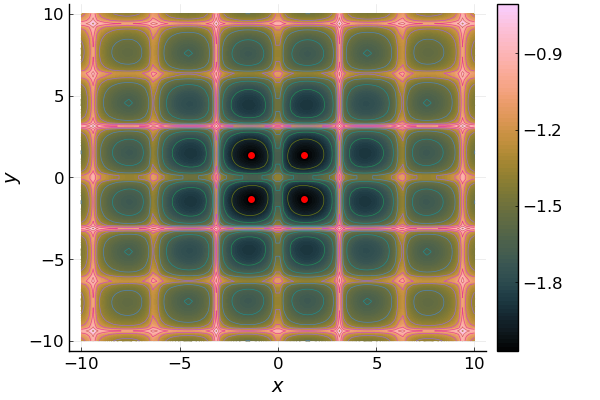
\includegraphics[width=\textwidth]
        {img/test_functions/cross_in_tray_contour.png}
      \caption{
        Contour plot showcasing the complex landscape of the Cross-in-Tray 
        function. 
        The red dot denotes the location of the global minimum.
      }
      \label{fig:app:test:cross-in-tray:contour}
    \end{subfigure}
    \hfill
    \begin{subfigure}[b]{0.45\textwidth}
      \centering
      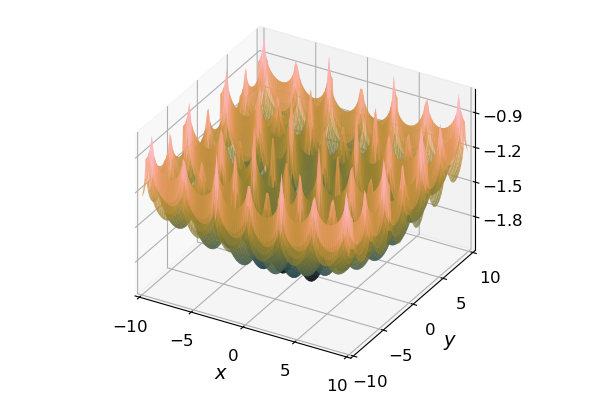
\includegraphics[width=\textwidth]
        {img/test_functions/cross_in_tray_surface.png}
      \caption{
        Surface plot providing a 3D representation of the Cross-in-Tray 
        function, enhancing the visualization of its global and local minima.
      }
      \label{fig:app:test:cross-in-tray:surface}
    \end{subfigure}
    \caption{
      Contour and surface plots illustrating the topological complexity of the 
      Cross-in-Tray function
    }
    \label{fig:app:test:cross-in-tray}
  \end{figure}
